\documentclass{beamer}
\usepackage[utf8]{inputenc}
\usetheme{Berkeley}
\setbeamertemplate{blocks}[rounded][shadow=true]
\usepackage{graphicx}
\usepackage{amsmath}
\usepackage{amssymb}
\usepackage{hyperref}
\usepackage{xcolor}
\usepackage{tikz}
\usetikzlibrary{tikzmark,positioning}

\makeatletter
\def\mathcolor#1#{\@mathcolor{#1}}
\def\@mathcolor#1#2#3{%
  \protect\leavevmode
  \begingroup
    \color#1{#2}#3%
  \endgroup
}
\makeatother

\definecolor{ForestGreen}{cmyk}{0.83,0.21,1,0.08}
\definecolor{ONTech-dark-blue}{cmyk}{1,0.58,0.09,0.46}
\definecolor{ONTech-light-blue}{cmyk}{1,0.31,0,0}
\definecolor{ONTech-orange}{cmyk}{0,0.70,1,0}
\definecolor{ONTech-warm-grey}{cmyk}{0.9,0.11,0.13,0.20}
\definecolor{ONTech-cool-grey}{cmyk}{0.20,0.14,0.12,0.40}
\definecolor{ONTech-dark-grey}{cmyk}{0.45,0.25,0.16,0.59}
\definecolor{ONTech-navy}{cmyk}{1,0.75,0.50,0.50}

% \renewcommand{\vec}[1]{\ensuremath{\boldsymbol{#1}}}
% \newcommand{\mtx}[1]{\ensuremath{\boldsymbol{#1}}}

\renewcommand{\vec}[1]{\ensuremath{\overline{#1}}}
\newcommand{\mtx}[1]{\ensuremath{\overline{\overline{#1}}}}
\newcommand{\vect}[1]{\ensuremath{\boldsymbol{#1}}}
 
%Information to be included in the title page:
\title{Multiphysics Reduced Order Modelling}
\subtitle{Reduced Basis Method for Lead-Cooled Fast Reactor}
\author{Parikshit Bajpai}
\date{MCSC 6020G - Numerical Analysis \\ \small{\today}}
 

\begin{document}
 
\frame{\titlepage}

\frame{\tableofcontents} 

\section{Motivation and Objectives}
\begin{frame}{Motivation}
\centering
\textbf{The full order simulation of nuclear reactors is extremely costly!}

Can we reduce the computational time and cost associated with these simulations without compromising with the accuracy?
\end{frame}

\begin{frame}{Objective}
\centering
Develop a Reduced Basis method, with basis functions sampled by a Proper Orthogonal Decomposition technique, to develop a reduced order model of a parametrised Lead-cooled Fast Reactor single-channel.
\end{frame}

\section{Background - Reactor Physics 00.01} 
\begin{frame}
\frametitle{Lead-cooled Fast Reactor (LFR)}
\begin{figure}
    \centering
    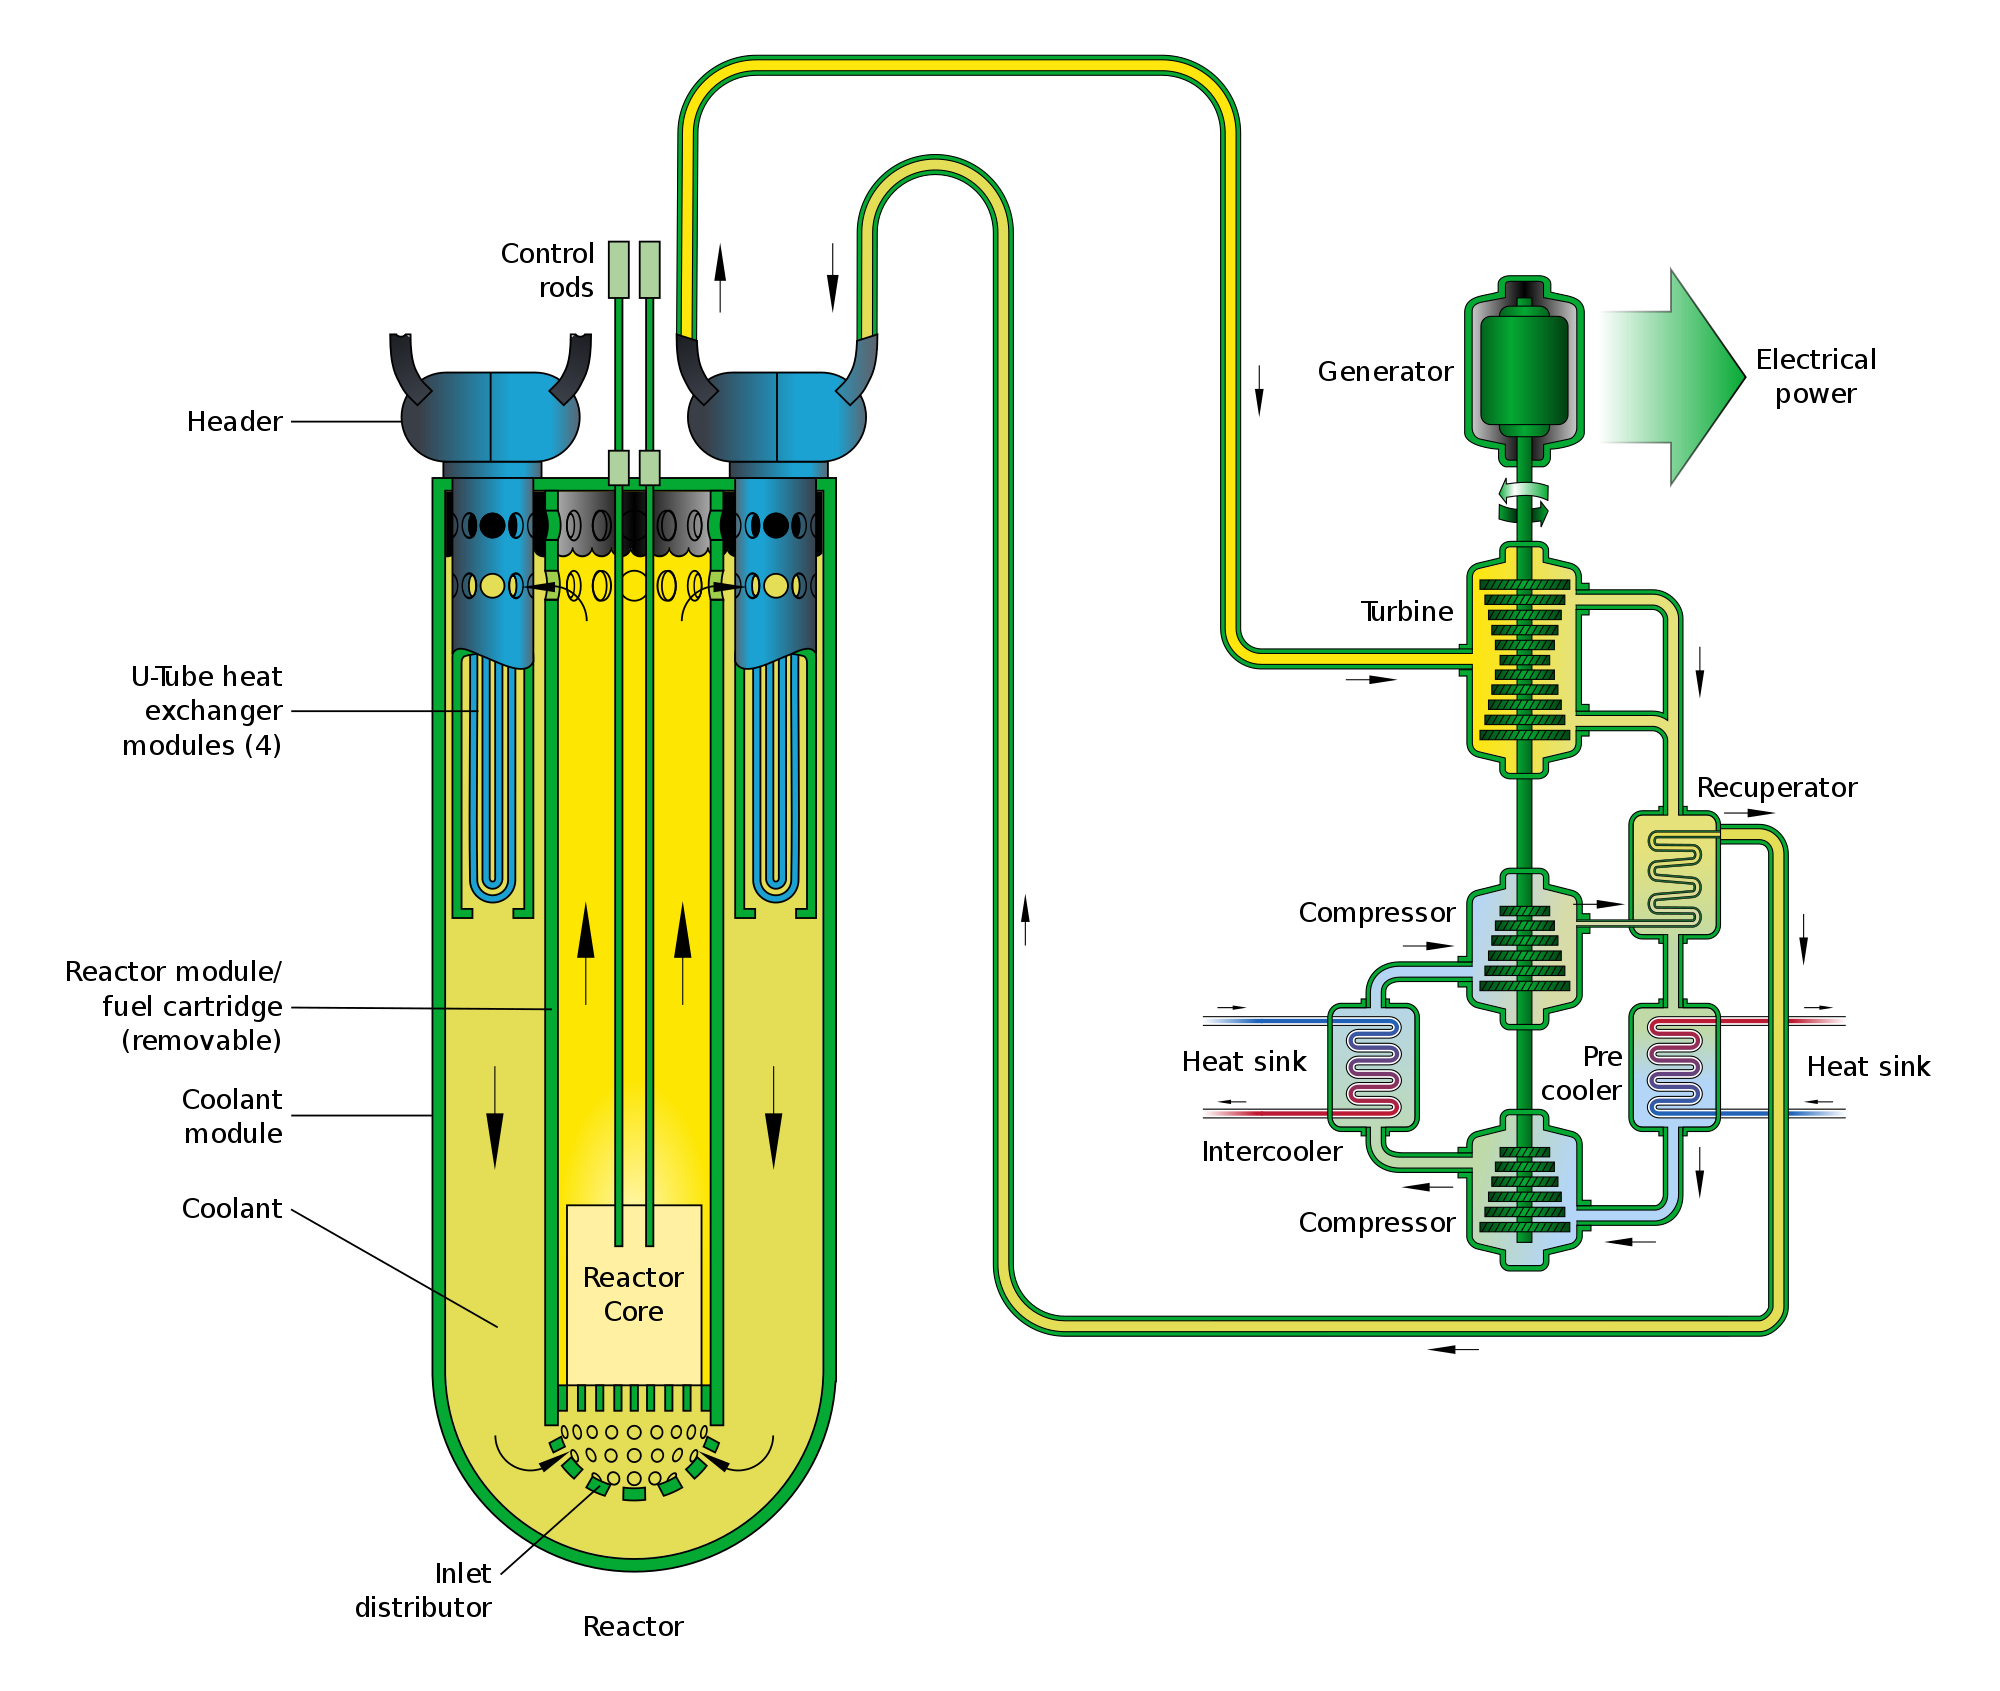
\includegraphics[width=0.8\textwidth]{LFR}
    \label{fig:LFR}
\end{figure}
\end{frame}

\begin{frame}
\frametitle{Neutron Flux}
\begin{block}{Neutron balance}
    \[
    \frac{\partial \phi}{\partial t} = -\mathcolor{red}{\nabla \cdot D \nabla \phi} + \mathcolor{ForestGreen}{\nu \Sigma_{f} \phi} - \mathcolor{red}{(\Sigma_{a} + \Sigma_{s} ) \phi}
    \]
\end{block}
    \bigskip
    \(\phi\) - Neutron Flux \\
    \(D\) - Diffusion Coefficient \\
    \(\Sigma_{a}\) - Macroscopic Absorption Cross Section \\
    \(\Sigma_{s}\) - Macroscopic Scattering Cross Section \\
    \(\nu\) - Fissile Yield (No. of neutrons produced per fission) \\
    \(\Sigma_{f}\) - Macroscopic Fission Cross Section \\
\end{frame}

\begin{frame}
\frametitle{Neutron Flux}
\begin{block}{}
    \[
    \tikzmark{bal} \frac{\partial \phi}{\partial t} = -\mathcolor{red}{\nabla \cdot \tikzmark{dif} D \nabla \phi} + \mathcolor{ForestGreen}{\nu \tikzmark{fis} \Sigma_{f} \phi} - \mathcolor{red}{(\Sigma_{a} + \Sigma_{s} )\phi \tikzmark{los}}
    \]
    
\begin{tikzpicture}[
    remember picture,
    overlay,
    expl/.style={draw=orange,fill=orange!30,rounded corners,text width=3.5cm,text centered},
    arrow/.style={red!80!black,ultra thick,->,>=stealth}
    ]
    \node<1->[expl] 
        (n01) 
        at (2,3cm)
        {Rate of change of neutron flux};
    \node<2->[expl] 
        (n02) 
        at (2,-2cm)
        {Diffusion of neutrons};
    \node<3->[expl] 
        (n03) 
        at (7.5,3cm)
        {Neutron production through fission};
    \node<4->[expl] 
        (n04) 
        at (7.5,-2cm)
        {Loss of neutrons due to absorption and scattering};
    \draw<1->[arrow]
        (n01) to[out=270,in=180] ([yshift=0.5ex]{pic cs:bal});
    \draw<2->[arrow]
        (n02) to[out=90,in=270] ([xshift=0.75ex,yshift=-0.5ex]{pic cs:dif});
    \draw<3->[arrow]
        (n03) to[out=270,in=90] ([xshift=0.75ex,yshift=2ex]{pic cs:fis});
    \draw<4->[arrow]
        (n04) to[out=90,in=360] ([xshift=0.25ex,yshift=0.5ex]{pic cs:los});
    \end{tikzpicture}
\end{block}
\end{frame}

\begin{frame}
\frametitle{Heat Transfer}
\begin{block}{Energy Balance}
    \[
    \frac{\partial T}{\partial t} = \mathcolor{ForestGreen}{\nabla \cdot [(K + K_T) \nabla T]} - \mathcolor{red}{\rho C_p \vect{v} \cdot \nabla T} + \mathcolor{ForestGreen}{Q}
    \]
\end{block}
    \bigskip
    \(T\) - Temperature \\
    \(K\) - Thermal Conductivity \\
    \(K_T\) - Turbulent Thermal Conductivity \\
    \(C_p\) - Heat Capacity \\
    \(\vect{v}\) - Velocity of fluid \\
    \(Q\) - Source Term \\
\end{frame}

\begin{frame}
\frametitle{Heat Transfer}
\begin{block}{}
    \[
    \tikzmark{bal} \frac{\partial T}{\partial t} = \mathcolor{ForestGreen}{\nabla \cdot [(K + \tikzmark{dif} K_T) \nabla T]} - \mathcolor{red}{\rho C_p \vect{v} \tikzmark{adv}\cdot \nabla T} + \mathcolor{ForestGreen}{Q \tikzmark{sor}}
    \]
    
\begin{tikzpicture}[
    remember picture,
    overlay,
    expl/.style={draw=orange,fill=orange!30,rounded corners,text width=3.5cm,text centered},
    arrow/.style={red!80!black,ultra thick,->,>=stealth}
    ]
    \node<1->[expl] 
        (n01) 
        at (2,3cm)
        {Rate of change of temperature};
    \node<2->[expl] 
        (n02) 
        at (2,-2cm)
        {Diffusion term};
    \node<3->[expl] 
        (n03) 
        at (7.5,3cm)
        {Advection term};
    \node<4->[expl] 
        (n04) 
        at (7.5,-2cm)
        {Source term};
    \draw<1->[arrow]
        (n01) to[out=270,in=180] ([yshift=0.5ex]{pic cs:bal});
    \draw<2->[arrow]
        (n02) to[out=90,in=270] ([xshift=0.75ex,yshift=-0.5ex]{pic cs:dif});
    \draw<3->[arrow]
        (n03) to[out=270,in=90] ([xshift=0.75ex,yshift=2ex]{pic cs:adv});
    \draw<4->[arrow]
        (n04) to[out=90,in=360] ([xshift=0.25ex,yshift=0.5ex]{pic cs:sor});
    \end{tikzpicture}
\end{block}
\end{frame}

\section{Parameterised Multiphysics Model} 
\begin{frame}{Multiphysics Model}
    \begin{figure}
        \centering
        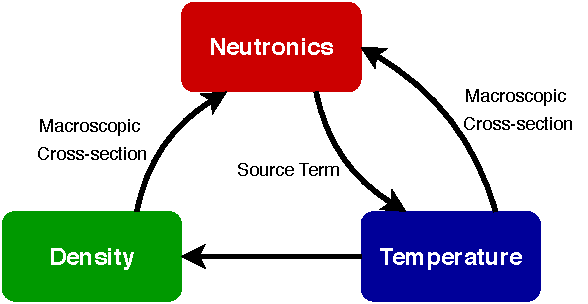
\includegraphics{Multiphysics.pdf}
    \end{figure}
\end{frame}

\begin{frame}{Parametrised Multiphysics Model}
    \begin{columns}
        \begin{column}{0.5\textwidth}
            \begin{itemize}
                \item Parametrised LFR single channel model.
                \item Rotational symmetry along fuel channel (r-z model).
                \item Time-independent settings.
                \item Parameters:
                    \begin{itemize}
                        \item Inner radius of fuel pellet $\mathcolor{blue}{\mu_1 \in [0.1, 0.43]} \text{ (cm)}$
                        \item Nominal coolant flow rate $\mathcolor{blue}{\mu_2 \in [0.8, 1.6]} \text{ (m/s)}$
                    \end{itemize}
            \end{itemize}
        \end{column}
        \begin{column}{0.5\textwidth} 
            \begin{center}
            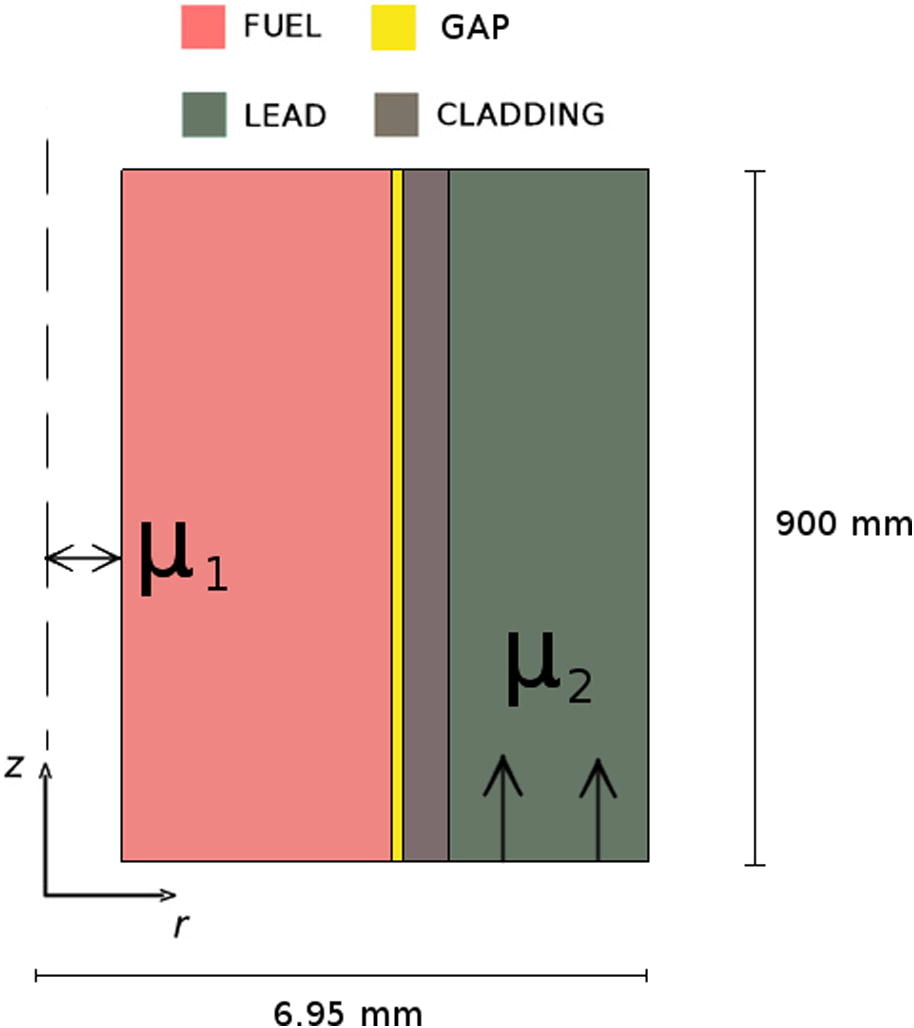
\includegraphics[width=\textwidth]{Parametric.jpg}
            \end{center}
        \end{column}
    \end{columns}
\end{frame}

\begin{frame}{Neutronics}
    The multi-group neutron diffusion equation in stationary formulation is a generalised eigenvalue problem. 
    \begin{block}{}
        \[\left ( - \nabla \cdot \mtx{D} \nabla + \mtx{\Sigma_a} + \mtx{\Sigma_s} \right ) \vec{\Phi} = \lambda_{eff} \vec{\chi} \vec{F}' \vec{\Phi}\]
    \end{block}
    \small
    \bigskip
    \begin{columns}
        \begin{column}{0.2\textwidth}
            \[
                \vec{\Phi} = 
                            \begin{bmatrix}
                                \Phi_1 (\mathbf{r}) \\
                                \vdots \\
                                \Phi_6 (\mathbf{r}) \\
                            \end{bmatrix}
            \]
        \end{column}
        \begin{column}{0.4\textwidth} 
            \[
                \mtx{D} = 
                            \begin{bmatrix}
                                D_1 (\mathbf{r}) & \dots & 0 \\
                                & \ddots & \\
                                & \dots & D_6 (\mathbf{r}) \\
                            \end{bmatrix}
            \]
        \end{column}
        \begin{column}{0.4\textwidth} 
                \[
                \mtx{\Sigma_a} = 
                            \begin{bmatrix}
                                \Sigma_a^1 (\mathbf{r}) & \dots & 0 \\
                                & \ddots & \\
                                & \dots & \Sigma_a^6 (\mathbf{r}) \\
                            \end{bmatrix}
            \]
        \end{column}
    \end{columns}
    \begin{columns}
        \hspace*{-2em}\begin{column}{0.625\textwidth}
            \[
                \mtx{\Sigma_s} = 
                            \begin{bmatrix}
                                \sum_{g' \neq 1}\Sigma_s^{1\rightarrow g'} (\mathbf{r}) & \dots & -\Sigma_s^{6\rightarrow 1} \\
                                & \ddots & \\
                                -\Sigma_s^{1\rightarrow 6} & \dots & \sum_{g' \neq 6}\Sigma_s^{6\rightarrow g'} \\
                            \end{bmatrix}
            \]
        \end{column}
        \begin{column}{0.1\textwidth} 
            \[
                \vec{\chi} = 
                            \begin{bmatrix}
                                \chi_1\\
                                \vdots \\
                                \chi_6\\
                            \end{bmatrix}
            \]
        \end{column}
        \begin{column}{0.15\textwidth} 
                \[
                \vec{F} = 
                            \begin{bmatrix}
                                \nu \Sigma_{f}^{1} (\mathbf{r})\\
                                \vdots \\
                                \nu \Sigma_{f}^{6} (\mathbf{r})\\
                            \end{bmatrix}
            \]
        \end{column}
        
    \end{columns}
\end{frame}

\begin{frame}{Neutronics}
    The multi-group neutron diffusion equation in stationary formulation is a generalised eigenvalue problem. 
    \begin{block}{}
        \[\left ( - \nabla \cdot \mtx{D} \nabla + \mtx{\Sigma_a} + \mtx{\Sigma_s} \right ) \vec{\Phi} = \lambda_{eff} \vec{\chi} \vec{F}' \vec{\Phi}\]
    \end{block}
    \bigskip
    \textbf{Fuel domain}
        \[\Sigma(T,\rho) = \frac{\rho}{\rho_0}\left[\Sigma_0 + \alpha \log\left(\frac{T}{T_0}\right)\right]\]
    \bigskip
    \textbf{Lead domain}
        \[\Sigma(T,\rho) = \frac{\rho}{\rho_0}\Sigma_0\]
\end{frame}

\begin{frame}{Neutronics}
    The multi-group neutron diffusion equation in stationary formulation is a generalised eigenvalue problem. 
    \begin{block}{}
        \[\left ( - \nabla \cdot \mtx{D} \nabla + \mtx{\Sigma_a} + \mtx{\Sigma_s} \right ) \vec{\Phi} = \lambda_{eff} \vec{\chi} \vec{F}' \vec{\Phi}\]
    \end{block}
    \bigskip
    \textbf{Boundary conditions}
    \begin{itemize}
        \item Albedo boundary conditions provide a good compromise between accuracy and computational requirements.
        \[\vec{n}\cdot(D_g\nabla \Phi_g) = - \gamma_z \phi_g\]
        \[\vec{n}\cdot(D_g\nabla \Phi_g) = - \gamma_r \phi_g\]
    \end{itemize}
\end{frame}

\begin{frame}{Heat Transfer}
    Within the cladding and gap domains the heat transfer is purely conductive. 
    \begin{block}{}
        \[-\nabla \cdot (K \nabla T) = 0\]
    \end{block}
    \bigskip
    Within the fuel domain the heat transfer is purely conductive but has a source term.
    \begin{block}{}
        \[-\nabla \cdot ( \nabla T) = \sum_{g=1}^{6}\Sigma_{g}^{f} E_f \Phi_g\]
    \end{block}
\end{frame}

\begin{frame}{Heat Transfer}
    Within the lead domain, the heat transfer is has an advective and a conductive term. 
    \begin{block}{}
        \[-\nabla \cdot \left [(K + K_T) \nabla T \right ]= \rho C_p \vect{v} \cdot \nabla T\]
    \end{block}
    \bigskip
    \textbf{Boundary conditions}
    \begin{itemize}
        \item Symmetry conditions at inner  radius of the fluid  domain and and outerradius of fluid domain.
        \item Homogeneous Neumann conditions on top and bottom of the domain.
    \end{itemize}
\end{frame}

\begin{frame}{Back to Objective}
    The full-fidelity model can have $\mathcal{O}(10^6 - 10^9)$ degrees of freedom.
    
    \bigskip
    We want to capture the behaviour of the system without using a high-fidelity, computationally expensive discretisation scheme.
\end{frame}

\begin{frame}{Offline/Online Strategy}
    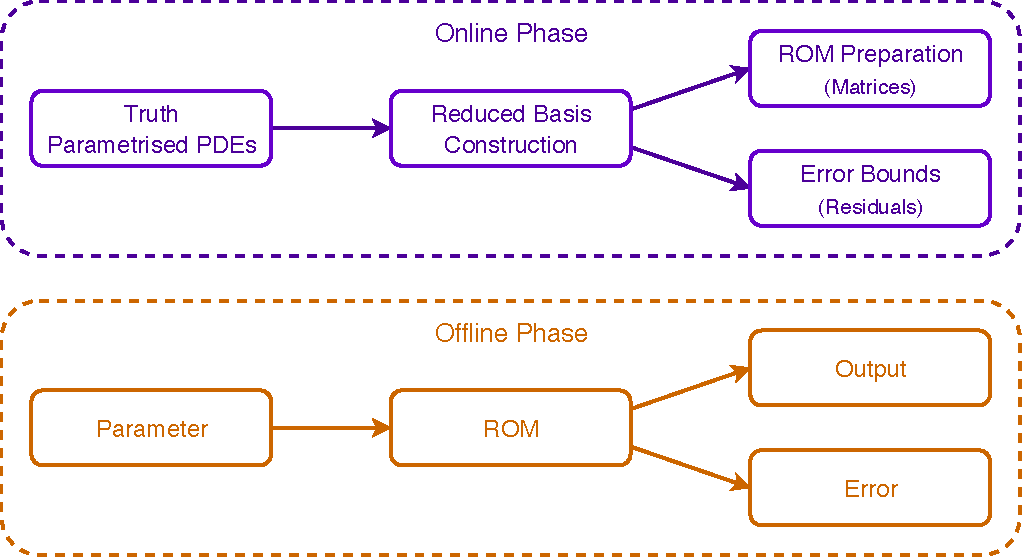
\includegraphics[width=\textwidth]{OLOF.pdf}
\end{frame}

\section{Finite Element Discretisation}
\begin{frame}{Finite Element Discretisation}
    \begin{block}{}
        For a given $\mu \in \mathcal{D}$, find $\vec{\Phi}(\mu) \in V^{\mathcal{N}}$ and $T(\mu) \in W^{\mathcal{N}}$ such that
        \[
        \mathrm{a}\left (\vec{\Phi},\vec{\nu}; \mu, \Sigma(T)\right ) = \lambda_{eff} \mathrm{m} \left (\vec{\Phi},\vec{\nu}; \mu, \Sigma(T)\right ) \mspace{30mu} \forall \vec{\nu} \in V^{\mathcal{N}}
        \]
        \[
        \mathrm{d}\left(T,w;\mu\right) = \mathrm{f}\left(w;\mu , S(\vec{\phi})\right) \mspace{30mu} \forall w \in W^{\mathcal{N}}
        \]
    \end{block}
    \begin{exampleblock}{}
        \begin{equation*}
            \begin{aligned}
            \mathrm{a}\left (\vec{\Phi},\vec{\nu}; \mu, \Sigma(T)\right ) = &\int_{\Omega} \mtx{D}(\nabla \vec{\Phi}\cdot\nabla\vec{\nu}) + (\mtx{\Sigma_a} + \mtx{\Sigma_s})\vec{\Phi}\vec{\nu} \\
            &+ \int_{\Gamma_{side}} \gamma_r \vec{\Phi}\vec{\nu} + \int_{\Gamma_{top} + \Gamma_{bot}} \gamma_z \vec{\Phi}\vec{\nu}
            \end{aligned}
        \end{equation*}
    \end{exampleblock}
    \begin{exampleblock}{}
        \begin{equation*}
            \mathrm{m} \left (\vec{\Phi},\vec{\nu}; \mu, \Sigma(T)\right ) = \int_{\Omega} \vec{\chi}\vec{F}'\vec{\Phi}\vec{\nu}
        \end{equation*}
    \end{exampleblock}
\end{frame}

\begin{frame}{Finite Element Discretisation}
    \begin{block}{}
        For a given $\mu \in \mathcal{D}$, find $\vec{\Phi}(\mu) \in V^{\mathcal{N}}$ and $T(\mu) \in W^{\mathcal{N}}$ such that
        \[
        \mathrm{a}\left (\vec{\Phi},\vec{\nu}; \mu, \Sigma(T)\right ) = \lambda_{eff} \mathrm{m} \left (\vec{\Phi},\vec{\nu}; \mu, \Sigma(T)\right ) \mspace{30mu} \forall \vec{\nu} \in V^{\mathcal{N}}
        \]
        \[
        \mathrm{d}\left(T,w;\mu\right) = \mathrm{f}\left(w;\mu , S(\vec{\phi})\right) \mspace{30mu} \forall w \in W^{\mathcal{N}}
        \]
    \end{block}
    \begin{exampleblock}{}
        \begin{equation*}
            \mathrm{d}\left(T,w;\mu\right) = \int_{\Omega} K \nabla T \nabla w  + \int_{\Omega_{lead}}  K_T \nabla T \nabla w
        \end{equation*}
    \end{exampleblock}
    \begin{exampleblock}{}
        \begin{equation*}
            \mathrm{f}\left(w;\mu , S(\vec{\phi})\right) = \int_{\Omega_{fuel}} Q w + \int_{\Omega_{lead}} \rho C_p (\vect{v}\cdot \nabla T) w
        \end{equation*}
    \end{exampleblock}
\end{frame}

\begin{frame}{Affine Parametric Dependence}
    \begin{exampleblock}{}
        \begin{equation*}
            \mathrm{a}\left (\vec{\Phi},\vec{\nu}; \mu, \Sigma(T)\right ) = \sum_{q=1}^{Q_a} \Theta_a^q (\mu) \mathrm{a}^q\left (\vec{\Phi},\vec{\nu}; \Sigma(T)\right )
        \end{equation*}
    \end{exampleblock}
    \begin{exampleblock}{}
        \begin{equation*}
            \mathrm{m} \left (\vec{\Phi},\vec{\nu}; \mu, \Sigma(T)\right ) = \sum_{q=1}^{Q_m} \Theta_m^q (\mu) \mathrm{m}^q \left (\vec{\Phi},\vec{\nu}; \Sigma(T)\right )
        \end{equation*}
    \end{exampleblock}
    \begin{exampleblock}{}
        \begin{equation*}
            \mathrm{d}\left(T,w;\mu\right) = \sum_{q=1}^{Q_d} \Theta_d^q (\mu) \mathrm{d}^q \left(T,w\right)
        \end{equation*}
    \end{exampleblock}
    \begin{exampleblock}{}
        \begin{equation*}
            \mathrm{f}\left(w;\mu , S(\vec{\phi})\right) = \sum_{q=1}^{Q_f} \Theta_f^q (\mu) \mathrm{f}^q\left(w; S(\vec{\phi})\right)
        \end{equation*}
    \end{exampleblock}
\end{frame}

\section{Reduced Basis Formulation}
\begin{frame}{Reduced Basis Model}
    \begin{block}{}
        The RB method is aimed at constructing reduced order solutions $\vec{\Phi}^{N_f}$ and $T^{N_T}$ such that
        \begin{equation*}
        \begin{aligned}
            \mathrm{a}\left (\vec{\Phi}^{N_f},\vec{\nu}; \mu, \Sigma(T^{N_T})\right ) = \lambda_{eff} \mathrm{m} \left (\vec{\Phi}^{N_f},\vec{\nu}; \mu, \Sigma(T^{N_T}) \right) \\ 
            \forall \vec{\nu} \in V^{N_f} \subset V^{\mathcal{N}}\\
        \end{aligned}
        \end{equation*}
        \begin{equation*}
        \begin{aligned}
        {\mathrm{d}\left(T^{N_T},w;\mu\right) = \mathrm{f}\left(w;\mu , S(\vec{\phi}^{N_f})\right)} \\ 
        \forall w \in W^{N_T} \subset W^{\mathcal{N}}
        \end{aligned}
        \end{equation*}
    \end{block}
\end{frame}

\begin{frame}{Reduced Basis Model}
    \begin{block}{}
        The RB method is aimed at constructing reduced order solutions $\vec{\Phi}^{N_f}$ and $T^{N_T}$ such that
        \begin{equation*}
        \begin{aligned}
            \mathrm{a}\left (\vec{\Phi}^{N_f},\vec{\nu}; \mu, \Sigma(T^{N_T})\right ) = \lambda_{eff} \mathrm{m} \left (\vec{\Phi}^{N_f},\vec{\nu}; \mu, \Sigma(T^{N_T}) \right) \\ 
            \forall \vec{\nu} \in V^{N_f} \subset V^{\mathcal{N}}\\
        \end{aligned}
        \end{equation*}
        \begin{equation*}
        \begin{aligned}
        {\mathrm{d}\left(T^{N_T},w;\mu\right) = \mathrm{f}\left(w;\mu , S(\vec{\phi}^{N_f})\right)} \\ 
        \forall w \in W^{N_T} \subset W^{\mathcal{N}}
        \end{aligned}
        \end{equation*}
    \end{block}
    The reduced spaces $V^{N_f}$ and $W^{N_T}$ have dimensions $N_f$ and $N_T$ respectively and are defined as:
    \[V^{N_f} = \mathrm{span}\left\{ \xi_1^f, \dots, \xi_{N_f}^f \right \} \mspace{20mu}
    W^{N_T} = \mathrm{span}\left\{ \xi_1^T, \dots, \xi_{N_T}^T \right \}\]
\end{frame}

\begin{frame}{Reduced Basis Model}
    \begin{exampleblock}{}
        \[{\Phi}^{N_f} = \sum_{i=1}^{N_f}\phi_{N,i}\xi_i^f \mspace{50mu} T^{N_T} = \sum_{j=1}^{N_T}T_{N,j}\xi_j^T\]
    \end{exampleblock}
    \begin{block}{}
        \[\mathrm{a}(\mathcal{Z}_f \vec{\phi_N},\vec{\nu};\mu,\Sigma(\mathcal{Z}_T \vec{T}_N)) = \lambda_{eff}^N \mathrm{m}(\mathcal{Z}_f \vec{\phi_N},\vec{\nu};\mu,\Sigma(\mathcal{Z}_T \vec{T}_N))\]
        \[\mathrm{d}(\mathcal{Z}_f \vec{T_N},w;\mu) = \mathrm{f}(w;\mu, S(\mathcal{Z}_f \vec{\phi_N}))\]
          \end{block}
    \begin{exampleblock}{}
        \[\mathcal{Z}_f = [\xi_1^f| \dots| \xi_{N_f}^f] \mspace{25mu} \mathcal{Z}_T = [\xi_1^T| \dots| \xi_{N_T}^T]\]
    \end{exampleblock} 
\end{frame}

\begin{frame}{Offline Phase}
\begin{block}{Offline}
    \begin{itemize}
        \item Run high fidelity computations to get snapshots.
        \item Construct matrices $\mathcal{Z}_f$ and $\mathcal{Z}_T$ required to build the matrices of ROM
        \item Matrices corresponding to the bilinear form of affine decompositions. 
    \end{itemize}
\end{block}

\begin{block}{Online}
    \begin{itemize}
        \item Multiply reduced matrices by proper coefficients and sum together.
        \item Solve the ROM.
    \end{itemize}
\end{block}
\end{frame}

\section{Expected Outcomes and Results}
\begin{frame}{Expected Outcomes and Results}
    \begin{itemize}
        \item Evaluate the errors between the reactivity provided by ROM and FE solution and error vs. number of basis functions.
            \[\epsilon_{\lambda}(\mu) = \left\vert\lambda_N(\mu) - \lambda_{\mathcal{N}}(\mu)\right\vert\]
        \item Evaluate the error between the neutron flux provided by the two models.
            \[\epsilon_{f} = \int_{\Omega}(\Phi^{N_f} - \vec{\Phi})^2\]
        \item Evaluate the error between the temperature field provided by the two models.
            \[\epsilon_{T} = \int_{\Omega}(T^{N_f} - {T})^2\]
    \end{itemize}
\end{frame}
\begin{frame}{Expected Outcomes and Results}
    \begin{itemize}
        \item Comparison of computational cost of ROM and FE model.
            \[\text{Speed-up} = \frac{\text{Wall time of ROM calculation}}{\text{Wall time of FE simulation}}\]
        \item Computational break-even.
            \[\text{Break-even} = \frac{\text{Total Offline time}}{\text{Time for 1 FE simulation}}\]
    \end{itemize}
\end{frame}
\begin{frame}{Sample Results}
   \begin{columns}
        \begin{column}{0.5\textwidth}
            \begin{center}
                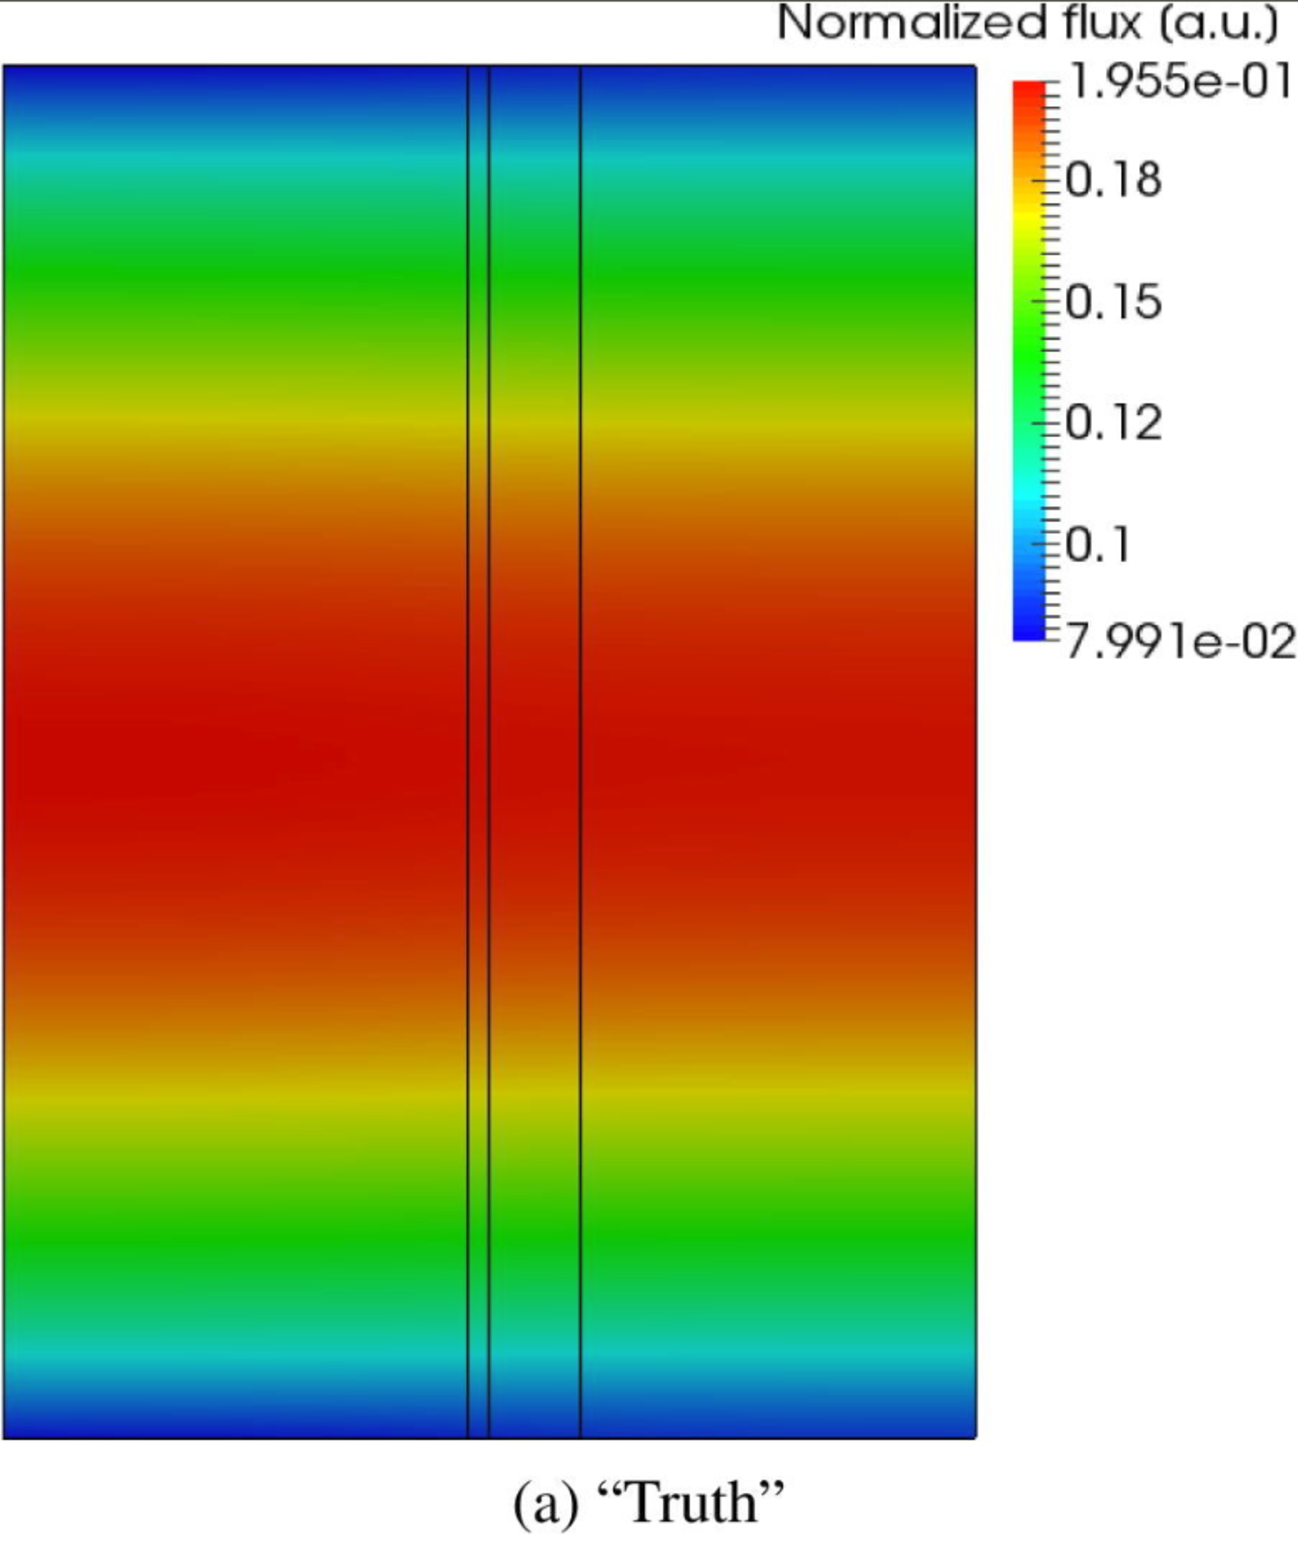
\includegraphics[width=\textwidth]{1.pdf}
            \end{center}
        \end{column}
        \begin{column}{0.5\textwidth} 
            \begin{center}
            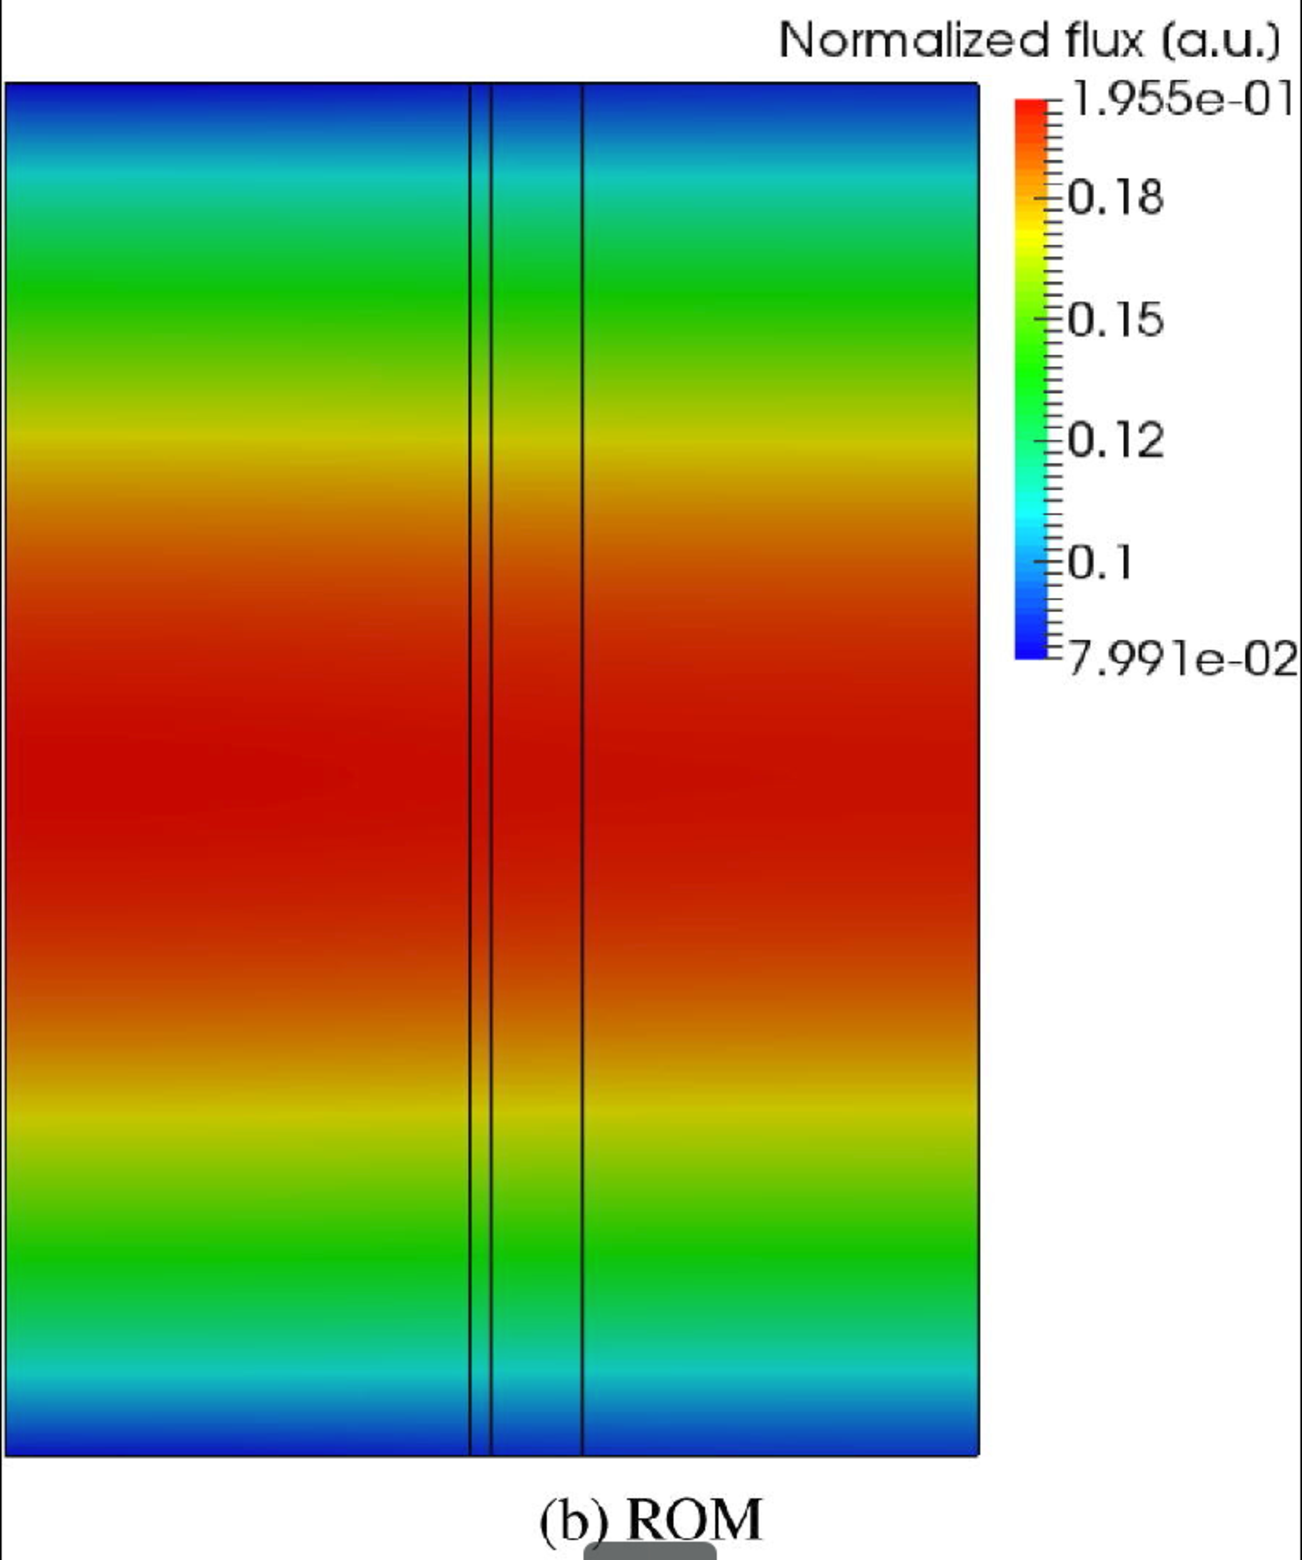
\includegraphics[width=\textwidth]{2.pdf}
            \end{center}
        \end{column}
    \end{columns}
\end{frame}

\begin{frame}{Sample Results}
            \begin{center}
                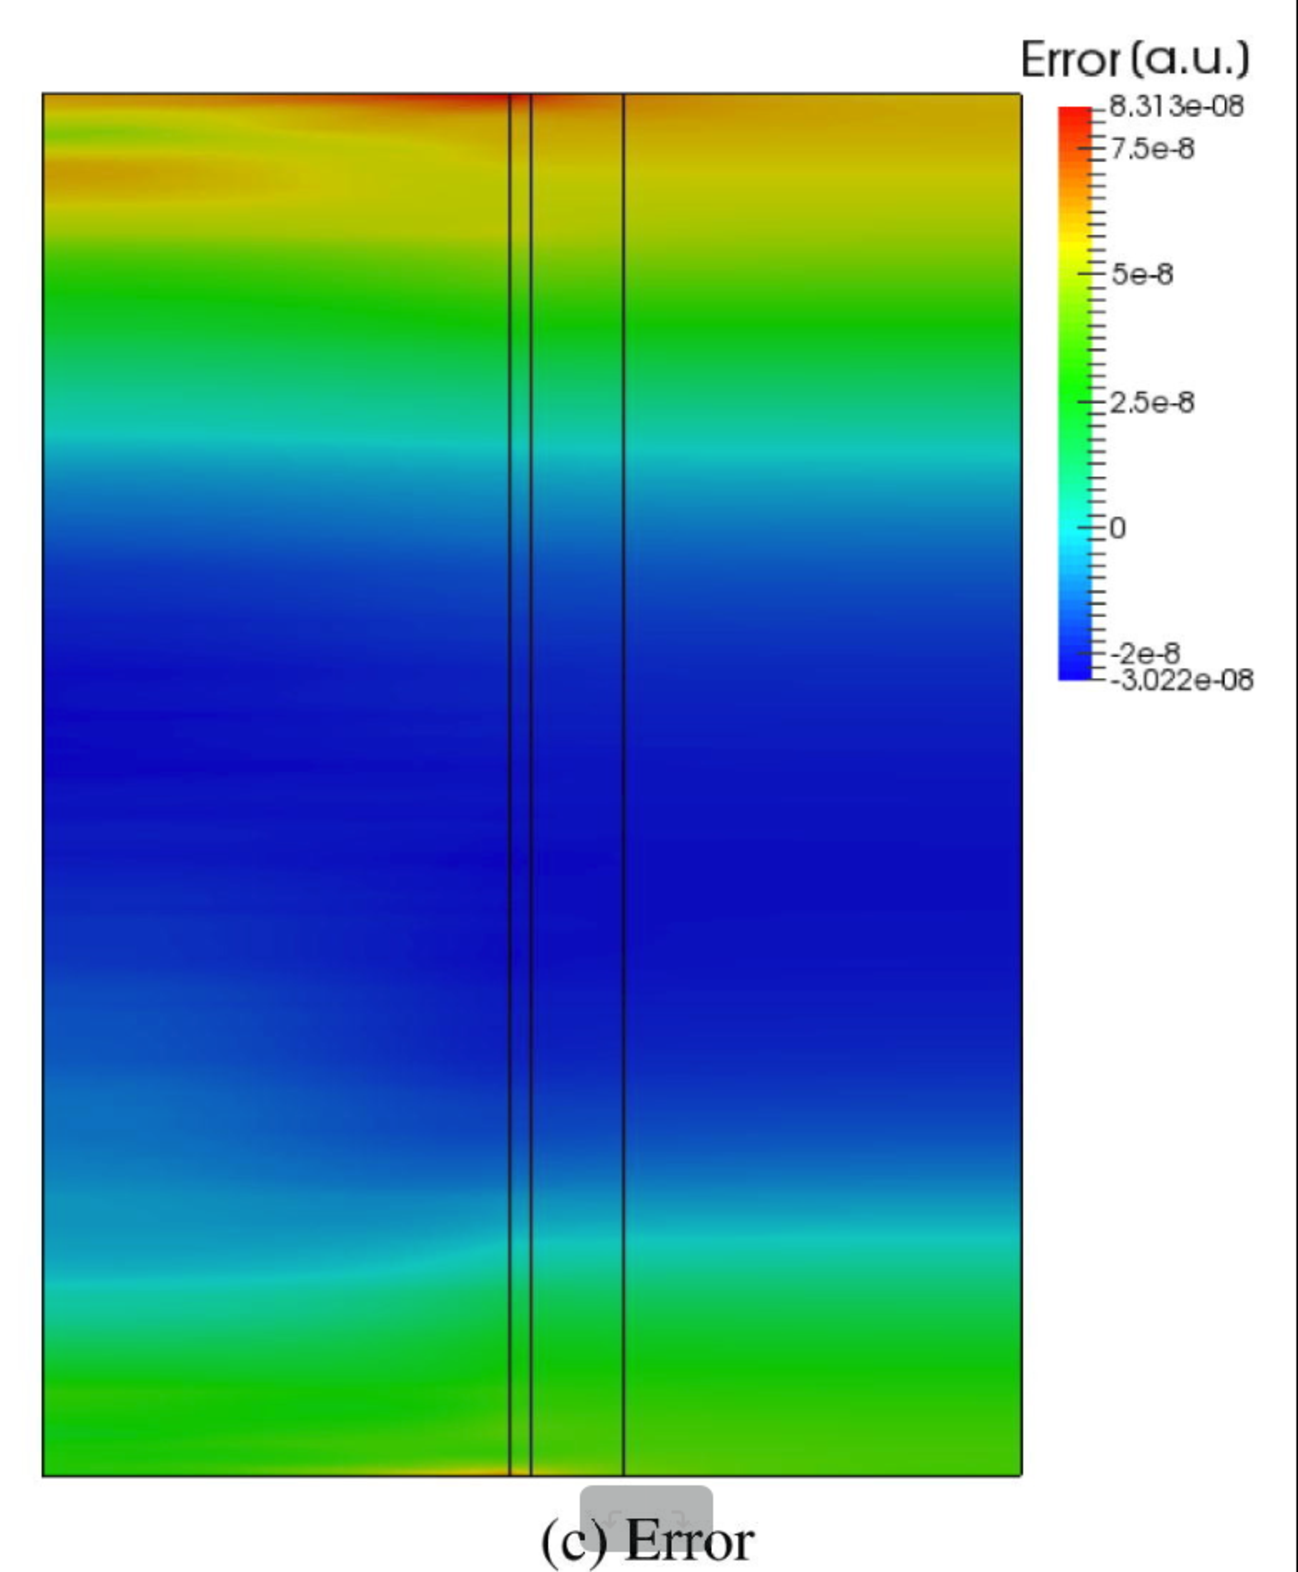
\includegraphics[width=0.5\textwidth]{3.pdf}
            \end{center}
       
\end{frame}
 
\end{document}